\documentclass[11pt]{article}

\usepackage[margin=1in]{geometry}
\usepackage{amsmath,amssymb,bm}
\usepackage{booktabs}
\usepackage{microtype}
\usepackage[table]{xcolor}
\usepackage{tikz}
\usetikzlibrary{arrows.meta,positioning,shapes.geometric,fit,backgrounds}
\usepackage[colorlinks=true,allcolors=blue!55!black]{hyperref}

\title{Routing the Silent Half:\\
       Per-Unit Choice of Estimator and Evolution Target in Self-Evolving LLM Agents}
\author{}
\date{}

\begin{document}
\maketitle

\begin{abstract}
Group-relative policy optimisation assigns zero advantage to any group whose samples score
alike, so a unanimous group contributes exactly nothing to the update. We measure this
directly: $57.4\%$ of groups in a live run are RL-silent. We show the silent half splits
into two regimes that require opposite responses, and that the split is not symmetric ---
on the solved half a supervised target is \emph{free}, because the group already contains a
correct sample; on the unsolved half no target exists unless one is supplied, which makes
harness evolution the only consumer that can use those units at all. We therefore make the
choice of estimator and the choice of evolution target a per-unit decision rather than a
per-run schedule, with the two as orthogonal axes so a single trajectory can feed both.
The closest prior work, DAPO's dynamic sampling, acts on exactly this set and responds in the
opposite way --- it discards the silent groups and oversamples to refill --- which on our own
measurements costs $1.5$--$2.4\times$ the rollouts, a multiplier that \emph{grows} with
training because the silent fraction itself grows from $0.33$ to $0.58$ on an arm with no
routing at all. We report the negative result that located this leverage: a token-level
version of the same idea, reaching $1.7\%$ of tokens, moved held-out accuracy by less than
the noise floor. Every capability is flag-gated and reduces to unmodified GRPO when disabled.
\end{abstract}

% ---------------------------------------------------------------------------
% Method. Formulas first, then the routing rule they imply, then the figure.
% ---------------------------------------------------------------------------
\section{Method}
\label{sec:method}

\subsection{Where the gradient is zero}
\label{sec:silence}

Let a \emph{unit} be a prompt with $G$ sampled answers and binary rewards
$r_1,\dots,r_G\in\{0,1\}$. GRPO centres rewards within the group,
%
\begin{equation}
  A_i \;=\; r_i - \bar r,
  \qquad
  \bar r \;=\; \frac{1}{G}\sum_{j=1}^{G} r_j ,
  \label{eq:adv}
\end{equation}
%
so if every sample in the group scores alike then $A_i=0$ for all $i$ and the unit
contributes exactly nothing to the update --- all $G$ sequences, every token. Writing
$p$ for the per-sample success probability, the probability that a unit carries any
signal at all is
%
\begin{equation}
  I_{\mathrm{RL}}(p,G) \;=\; 1 - p^{G} - (1-p)^{G},
  \label{eq:irl}
\end{equation}
%
which is zero exactly at $p=0$ and $p=1$ and is maximised at $p=\tfrac12$. Equation
\eqref{eq:irl} is not an approximation: it is the probability that the group is not
unanimous, and unanimity is precisely the condition under which \eqref{eq:adv} vanishes.

Two consequences drive the method.

\paragraph{The silent fraction is large and measurable.} Instrumenting a live run
(Sec.~\ref{sec:results}) puts $\hat{P}(\text{silent})$ between $0.29$ and $0.57$ depending on
the training step, at $64$ groups per batch: a third to a half of every batch is RL-dead.
Even the low end is an order of magnitude above the reach of the token-level shared-prefix
channel we measured first ($1.7\%$), and that gap explains, without appealing to noise, why
an intervention confined to that channel moved nothing.

\paragraph{The two silent regimes need opposite responses, and they are not equally
common.} A unit silent because $\hat p = 1$ and a unit silent because $\hat p = 0$ are both
invisible to \eqref{eq:adv}, but they are not the same object, and routing them identically
wastes one of them. Measured on the control arm, the silent channel is $87.5\%$ solved
(Table~\ref{tab:split}), which decides which of the two branches carries the method.

\paragraph{The composition is a property of the task \emph{and} the model, and it moves in both
directions.} The $87.5\%$ is GSM8K with Qwen2.5-1.5B-Instruct; on MATH, holding the model
fixed, it inverts to $39.1\%$ solved and $60.9\%$ unsolved (Table~\ref{tab:flip}). Re-measured
on the arm this paper trains --- decontaminated DeepMath with Qwen2.5-32B-Instruct, over $245$
logged steps of the baseline --- the channel is $0.505$ of all groups and splits $0.338$ solved,
$0.167$ unsolved and $0.000$ unclassified, i.e.\ $66.9\%$ solved and $33.1\%$ unsolved. The
unsolved share is therefore roughly \emph{half} what the MATH column reports, and we state the
confound plainly: that pair varies the model as well as the task, so it cannot separate a
task effect from a scale effect, and both readings shrink the branch. Two consequences are load
bearing. First, any statement sized on the $60.9\%$ figure must not be carried onto this arm:
the unsolved branch is about a sixth of every batch here, not a third. Second, the
$0.000$ unclassified mass means no group on this arm is silent for a reason the correctness
split cannot express, so unlike on GSM8K the composition ratio has a clean denominator and
$\text{unsolved}/\text{silent}$ and $\text{unsolved}/(\text{solved}+\text{unsolved})$ coincide.

\subsection{A free target exists on exactly the solved half}
\label{sec:selftarget}

The asymmetry is sharper than "different regimes''. For a unit with $\hat p > 0$, at least
one sampled answer was correct, and that answer \emph{is} a supervised target drawn from
the model's own rollout. No external teacher is required; this is rejection-sampling
fine-tuning. Define
%
\begin{equation}
  \mathrm{selfTarget}(u) \;=\; \mathbb{1}\!\left[\hat p_u > 0\right],
  \qquad
  \mathrm{target}(u) \;=\; \mathrm{selfTarget}(u) \;\vee\; \mathrm{teacher}(u).
  \label{eq:target}
\end{equation}
%
The units on which $I_{\mathrm{RL}}=0$ because $\hat p = 1$ are therefore exactly the units
on which a target is \emph{guaranteed} to exist at zero marginal cost. The units on which
$I_{\mathrm{RL}}=0$ because $\hat p = 0$ are exactly the units on which no target exists
unless one is supplied. The gradient-free half of the batch splits cleanly into a half that
is free to reuse and a half that is not reusable at all.

\subsection{Supplying a target for the half that has none}
\label{sec:supply}

``Not reusable at all'' is a statement about \eqref{eq:adv}, not about the batch. An advantage
is a coefficient on tokens the model \emph{emitted}, so on a unit with $\hat p = 0$ every value
that could be written into the advantage tensor multiplies a wrong derivation, and a positive
constant there is a step toward the error --- which is why $c_- \le 0$ is required and why no
router in our registry reaches this branch. The only altitude at which a correct row can receive
gradient is \emph{batch construction}: put the correct response in as a row, with its own prompt
and its own loss mask, and the estimator that already runs on every other row runs on it too.
This is the construction of LUFFY and of DyME, and it is what makes the unsolved branch
addressable at all.

\paragraph{The supplier is an axis, not a constant.} Once the row enters by construction, where
it came from is a separate question from where it goes: the splice, the masks, the counters and
the off-policy treatment are properties of inserting a correct row and do not depend on its
origin. We therefore define a supplier interface with four implementations --- the dataset's
gold solution; a \emph{self-generated} correct rollout of the same prompt from an earlier step
or a higher-temperature resample; a row from an offline \emph{corpus} of solved examples; and a
verified completion from a stronger \emph{teacher} --- and route a unit to one of them. Prompt
identity is derived from the prompt tokens rather than from a batch-local index, because a
self-generated row is by definition one the same prompt received at a different step.

\paragraph{A supplier that has nothing must refuse, and the refusal is the measurement.} Each
supplier either returns token ids or raises a typed refusal, and every reason has its own
counter that is reported whether or not it is zero: a missing dataset solution, a prompt never
solved before, a derivation too long for the row, and a teacher completion that fails
verification have four different remedies, and a single ``skipped'' total sends the reader to
the wrong one. No supplier substitutes a row belonging to a different prompt, and no supplier
truncates: a cut-off derivation is a wrong target that still looks like a target. The teacher
requires an explicit verifier for the same reason --- a stronger model is not a correct one, and
this is precisely the branch on which nothing else would catch the error.

\paragraph{The source decision is fixed, and its control is not optional.} The choice of
supplier is expressible per unit, but we do not learn it here. We use an explicit ordered
policy, cheapest-and-most-trusted first, and compare it against a control that replays the
policy's own realised source assignment permuted across units, so the mixture of sources is
matched exactly by construction and only the \emph{targeting} differs. This is the same
falsification the routing control performs one axis over, and we run it for the same reason: in
this project a learned mechanism has repeatedly matched a feature-blind control at matched
proportions once the control was finally run, and a claim about choosing sources that has not
been separated from a claim about mixing them is not a claim.

\subsection{Routing: the harness is a destination, not a schedule}
\label{sec:routing}

Prior work treats the choice of what to evolve as a property of the \emph{run}: a schedule
or a global flag. We make it a property of the \emph{unit}, and we make it two-dimensional.
A routing decision is a pair
%
\begin{equation}
  \pi(u) \;=\; \bigl(m(u),\, h(u)\bigr),
  \qquad
  m \in \{\textsc{rl}, \textsc{sft}, \textsc{skip}\},
  \qquad
  h \in \{\textsc{none}, \textsc{propose}, \textsc{validate}\},
  \label{eq:action}
\end{equation}
%
where $m$ names the estimator applied to the unit's tokens and $h$ names what the unit
contributes to harness evolution. The two axes are orthogonal by construction, so a single
trajectory can feed the gradient and the harness at once. This is deliberate: the two
consumers read different things from a trajectory --- the estimator reads the tokens, the
harness evolver reads the failure mode --- and a partition discards one of the readings.
Co-Harness's success$\to$model / failure$\to$harness rule is the special case in which
$\pi$ is constrained to be a partition, and we retain it as an ablation
(\texttt{partition=True}) rather than a rewrite.

The rule implied by \eqref{eq:irl} and \eqref{eq:target} is then forced rather than chosen:
%
\begin{equation}
  \pi(u) \;=\;
  \begin{cases}
    (\textsc{sft}_{\text{self}},\ \textsc{validate})
      & \hat p_u = 1 \quad\text{(RL dead; target free)}\\[2pt]
    (\textsc{sft}_{\text{teacher}},\ \textsc{propose})
      & \hat p_u = 0 \ \wedge\ \mathrm{teacher}(u) \\[2pt]
    (\textsc{skip},\ \textsc{propose})
      & \hat p_u = 0 \ \wedge\ \neg\,\mathrm{teacher}(u)
      \quad\text{(harness is the only consumer)}\\[2pt]
    (\textsc{rl},\ \textsc{none})
      & 0 < \hat p_u < 1 \quad\text{(RL has signal; leave it alone)}
  \end{cases}
  \label{eq:rule}
\end{equation}
%
Note the third case. When a unit is unsolved and no teacher is available, the model arm has
nothing to learn from it, and any method that only evolves weights must discard the unit.
Routing it to the harness is what makes it recoverable at all, which is the concrete sense
in which the harness axis is not a convenience.

\paragraph{One trajectory, two consumers.} \eqref{eq:rule} as written still couples the two
axes: a unit that RL can learn from contributes nothing to the harness. That is a residual
partition, and it discards information --- a \emph{mixed} unit contains failed samples, and
their failure mode is exactly what a harness evolver reads, while the RL update consumes only
the reward. We therefore decouple the harness action with its own threshold $\tau_h$:
%
\begin{equation}
  h(u) \;=\;
  \begin{cases}
    \textsc{validate} & \hat p_u = 1 \\
    \textsc{propose}  & \hat p_u \le \tau_h \\
    \textsc{none}     & \text{otherwise,}
  \end{cases}
  \qquad \tau_h \ge \tau_{\text{fail}} ,
  \label{eq:harness}
\end{equation}
%
so at $\tau_h = \tau_{\text{fail}}$ the rule is unchanged, and raising it lets a unit take
$(\textsc{rl}, \textsc{propose})$ --- feeding the gradient and the harness from the same
trajectory. Under $\texttt{partition}$ this is disabled, so the Co-Harness special case is
preserved exactly.

\paragraph{Rollback.} Every capability above is gated. With the harness arm disabled,
$h(u) \equiv \textsc{none}$; with routing disabled, $\pi(u) \equiv (\textsc{rl},
\textsc{none})$ for every unit and the update is bit-identical to unmodified GRPO; with the
supplier axis of Sec.~\ref{sec:supply} disabled, the batch construction reduces to its single
original source and its output is byte-identical, key set included, which we verify against a
digest recorded before the generalisation existed rather than by inspection. Each
ablation in Sec.~\ref{sec:results} is one flag away from the vanilla baseline, so a
difference cannot be attributed to an incidental change of configuration.



\subsection{Who decides: from a threshold to a controller}
\label{sec:controller}

Everything above specifies an action space. What chooses within it is a separate question,
and it is where the contribution lies --- a rule keyed on $\hat p$ is a heuristic, and a
learned policy that sees only $\hat p$ cannot beat the best threshold on $\hat p$ by more
than noise. We therefore give the controller features, and instantiate it three ways so the
comparison is an ablation rather than a demonstration.

\paragraph{Features, at zero marginal cost.} Each unit is described by seven statistics
computed from tensors the batch \emph{already carries} --- rewards, the loss mask, and the
sampled log-probabilities. No extra forward pass, no extra generation. The constraint is
deliberate: a feature set needing its own inference budget would have to beat spending that
budget on more rollouts, which is a far higher bar than beating a threshold. Two of the seven
carry information $\hat p$ cannot: the \emph{truncated fraction} separates a unit that failed
from one that merely ran out of budget, and the \emph{log-probability dispersion} separates a
group unanimous in its answer from one also unanimous in its reasoning. A solve-rate
threshold collapses both distinctions by construction.

\paragraph{Three controllers, one action space.}
%
\begin{itemize}
  \item \textbf{Rule} --- thresholds on $\hat p$, as in \eqref{eq:rule}. The baseline the
        others must beat, not a strawman: it encodes the exact zero-gradient condition.
  \item \textbf{Learned weights} --- LinUCB, one ridge model per mode over the features,
        updated from observed outcomes. Ridge rather than a network because the outcome
        channel is confounded and low-signal --- one scalar per batch, produced by every
        decision in it --- and capacity would mostly fit that noise.
  \item \textbf{Learned code} --- the policy is generated \emph{source}, validated against an
        allowlist and cost-vetted in a subprocess before adoption. Strictly larger
        hypothesis class than weights: it can compose features into ratios and nested cases
        rather than only reweighting them.
\end{itemize}
%
\paragraph{The control that decides the claim.} A fourth arm shuffles which units receive
which mode while holding the \emph{proportion} of units in each mode fixed. Without it, a
controller that helps cannot be distinguished from a change in how much SFT the run did ---
and the latter is not a controller at all. Any improvement reported for the learned arms is
the improvement over this control, not over the fixed rule alone.

\paragraph{What we verify about the learned arm, and what we do not.} On a synthetic
environment whose two regions differ \emph{only} in the truncated fraction, with $\hat p$
held identical, the contextual controller reaches the optimal mode in both regions across
seeds, while a context-free bandit on the same stream provably cannot exceed $0.5$ in the
worse region. That establishes the mechanism can use a feature a threshold cannot see. It
does \emph{not} establish that it learns under the confounded batch-level channel of a real
run, which is a separate claim and is not made here.

\subsection{The procedure, end to end}
\label{sec:algo}

Algorithm~\ref{alg:route} is the whole method. Every line is either an existing GRPO step or
a decision from \eqref{eq:rule}--\eqref{eq:harness}; nothing else is added, and with routing
disabled lines 6--13 do not execute.

\begin{algorithm}[t]
\caption{Per-batch signal routing. $\mathcal{B}$ is a batch of prompts, $G$ samples each.}
\label{alg:route}
\begin{algorithmic}[1]
\Require thresholds $\tau_{\text{solve}}{=}1$, $\tau_{\text{fail}}{=}0$, $\tau_h \ge \tau_{\text{fail}}$;
         weights $c_+ \ge 0$, $c_- \le 0$; flags \texttt{routing}, \texttt{harness}
\State roll out $G$ samples per prompt; score to binary rewards $r_{u,i}$
\State $\hat p_u \gets \frac{1}{G}\sum_i r_{u,i}$ \Comment{group solve rate}
\State $A_{u,i} \gets r_{u,i} - \hat p_u$ \Comment{group-centred advantages, \eqref{eq:adv}}
\State $\mathcal{S} \gets \{u : \max_i |A_{u,i}| = 0\}$ \Comment{RL-silent: exactly the unanimous units}
\If{\texttt{routing}}
  \ForAll{$u \in \mathcal{S}$}
    \If{$\hat p_u \ge \tau_{\text{solve}}$} \Comment{solved: a correct sample is its own target}
      \State $A_{u,i} \gets A_{u,i} + c_+$ for all response tokens
    \ElsIf{$\hat p_u \le \tau_{\text{fail}}$} \Comment{failed: no self-target exists}
      \State $A_{u,i} \gets A_{u,i} + c_-$ \textbf{if} $c_- \neq 0$, else leave at $0$
    \EndIf
  \EndFor
\EndIf
\If{\texttt{harness}}
  \State $\mathcal{P} \gets \{u : \hat p_u \le \tau_h\}$; \; $\mathcal{V} \gets \{u : \hat p_u = 1\}$
  \State emit $(\textsc{propose}, u)$ for $u \in \mathcal{P}$ and $(\textsc{validate}, u)$ for $u \in \mathcal{V}$
\EndIf
\State PPO update on $\{A_{u,i}\}$, clipping unchanged
\end{algorithmic}
\end{algorithm}

\paragraph{Why the update needs no new loss term.} Line 8 is the whole of the supervised
branch. For a solved unit every $A_{u,i}$ is zero, so adding $c_+$ makes the objective
$c_+\sum_i \log \pi(y_{u,i})$ over samples already known to be correct --- which is supervised
fine-tuning on them, with the importance ratio at $1$ because the data is on-policy. PPO's
clip still bounds the step, which matters because sharpening an already-correct policy is the
mechanism's predicted failure. Line 10 is its mirror: $c_- \le 0$ pushes down samples known to
be wrong, and $c_- > 0$ is rejected rather than trusted, since it would train the model to
reproduce them.

\paragraph{Cost.} Lines 5--13 add no generation. The batch is the batch that GRPO already
rolled out; the silent units are re-read, not re-sampled. This is the whole of the difference
from DAPO, which reaches the same set by discarding it and paying to generate a replacement.

% Method flowchart. Standalone-compatible: the same TikZ source is exported to SVG by
% scripts/build_figs.sh, so the figure in the paper and the figure on the web are one file.
\begin{figure}[t]
\centering
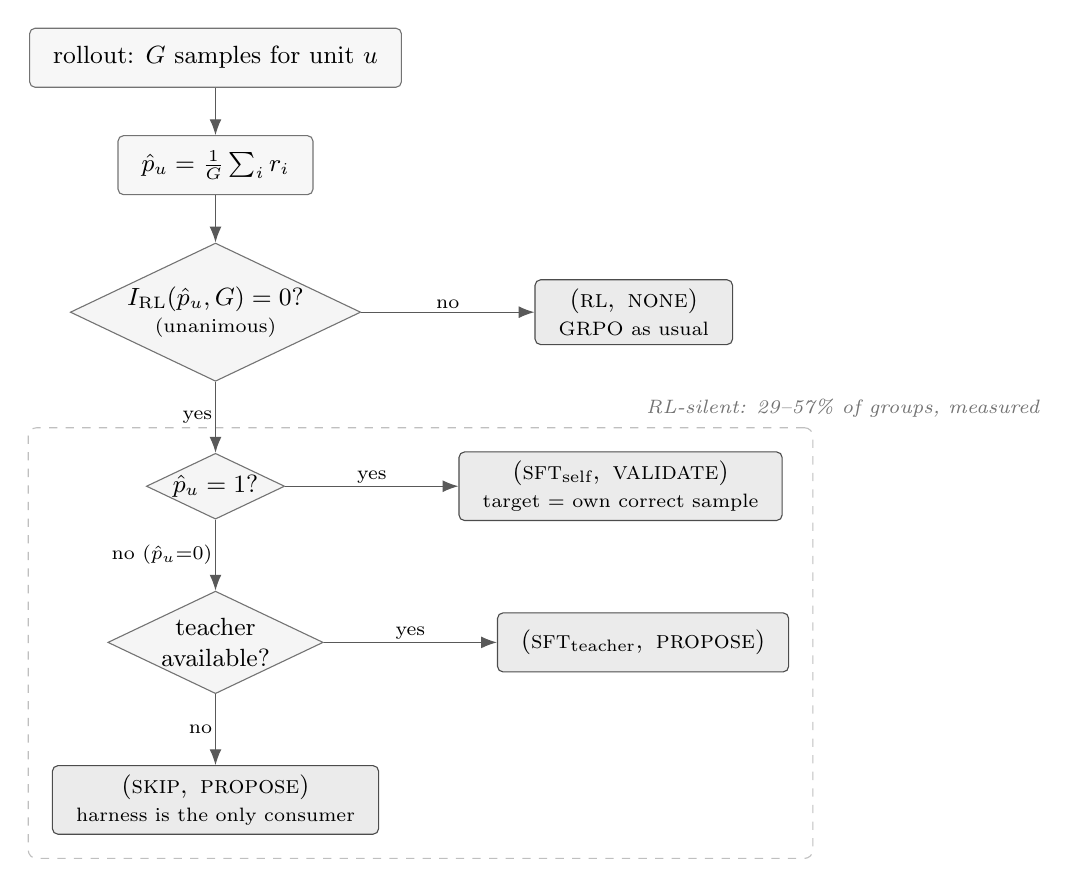
\begin{tikzpicture}[
  font=\small,
  node distance=6mm and 9mm,
  box/.style   ={rectangle, rounded corners=2pt, draw=black!55, fill=black!3,
                 minimum height=7.5mm, inner xsep=3mm, align=center},
  test/.style  ={diamond, aspect=2.1, draw=black!55, fill=black!4,
                 inner xsep=0.4mm, inner ysep=0mm, align=center},
  sink/.style  ={rectangle, rounded corners=2pt, draw=black!70, fill=black!8,
                 minimum height=7.5mm, inner xsep=3mm, align=center},
  arr/.style   ={-{Latex[length=2mm]}, draw=black!65},
  lbl/.style   ={font=\scriptsize, inner sep=1pt, fill=white}
]

\node[box] (roll) {rollout: $G$ samples for unit $u$};
\node[box, below=of roll] (rate) {$\hat p_u=\frac1G\sum_i r_i$};
\node[test, below=of rate] (sil) {$I_{\mathrm{RL}}(\hat p_u,G)=0$?\\[-1pt]\scriptsize(unanimous)};

\node[sink, right=22mm of sil] (rl) {$(\textsc{rl},\ \textsc{none})$\\[-1pt]\scriptsize GRPO as usual};

\node[test, below=9mm of sil] (solved) {$\hat p_u = 1$?};
\node[sink, right=22mm of solved] (sft) {$(\textsc{sft}_{\text{self}},\ \textsc{validate})$\\[-1pt]\scriptsize target = own correct sample};

\node[test, below=9mm of solved] (tea) {teacher\\available?};
\node[sink, right=22mm of tea] (sftt) {$(\textsc{sft}_{\text{teacher}},\ \textsc{propose})$};
\node[sink, below=9mm of tea] (skip) {$(\textsc{skip},\ \textsc{propose})$\\[-1pt]\scriptsize harness is the only consumer};

\draw[arr] (roll) -- (rate);
\draw[arr] (rate) -- (sil);
\draw[arr] (sil)   -- node[lbl,above]{no} (rl);
\draw[arr] (sil)   -- node[lbl,left]{yes} (solved);
\draw[arr] (solved)-- node[lbl,above]{yes} (sft);
\draw[arr] (solved)-- node[lbl,left]{no ($\hat p_u{=}0$)} (tea);
\draw[arr] (tea)   -- node[lbl,above]{yes} (sftt);
\draw[arr] (tea)   -- node[lbl,left]{no} (skip);

\begin{scope}[on background layer]
  \node[draw=black!25, dashed, rounded corners=3pt, fit=(solved)(tea)(skip)(sftt)(sft),
        inner sep=3mm, label={[font=\scriptsize\itshape, black!55]above right:%
        RL-silent: 29--57\% of groups, measured}] {};
\end{scope}
\end{tikzpicture}
\caption{%
  \textbf{Routing decides, per unit, both an estimator and a harness contribution.}
  The branch on $I_{\mathrm{RL}}$ is exact, not heuristic: a unanimous group has every
  advantage identically zero by \eqref{eq:adv}. The dashed region is the part of the batch
  ordinary GRPO cannot learn from, measured at $29$--$57\%$ of groups depending on training
  step. It does not split evenly: $87.5\%$ of it is solved, where a supervised target is
  free (the unit's own correct sample), and the remainder has no target unless one is
  supplied --- and on that remainder the harness is the only consumer that can use the unit
  at all.}
\label{fig:routing}
\end{figure}


% ---------------------------------------------------------------------------
% Related work, organised by what each line of work OWNS, so the contribution is
% stated as a gap rather than as a list.
% ---------------------------------------------------------------------------
\section{Related work}
\label{sec:related}

We organise prior work by the claim it already owns, because our contribution is only
meaningful as the complement of those claims.

\paragraph{Choosing an algorithm per task.} SIA selects among training algorithms at the
granularity of a \emph{task}, and demonstrates that the choice matters. That result is
theirs and we do not re-derive it. What a task-level policy cannot express is that units
\emph{within} one task differ in whether a gradient exists at all: by \eqref{eq:irl} the
silent and informative units of a single task require different estimators, and no
task-level assignment can separate them. Our claim is therefore about granularity, and the
comparison that matters is against SIA at matched compute.

\paragraph{Deciding what to evolve.} Co-Harness co-evolves harness and weights and
establishes the success$\to$model / failure$\to$harness assignment. EvoTrainer co-evolves a
policy with its training harness. Both fix the assignment as a rule over outcomes. We keep
their rule as a special case (\eqref{eq:action} constrained to a partition) and relax it,
because a trajectory read by two different consumers need not be spent on only one of them.

\paragraph{Deciding \emph{when} to evolve.} \emph{Learning, Fast and Slow} separates fast
and slow adaptation and reports the stability benefit of a two-timescale schedule. That
bounds what a cadence claim can be worth, and we treat cadence as a control variable rather
than a contribution.

\paragraph{Clustering trajectories.} MEDS reuses layer-wise logits from the forward pass as
lightweight representations of reasoning behaviour and clusters error patterns with HDBSCAN.
We adopt this directly as the learned instantiation of our cluster key, against a derived
key computed from the silence side of \eqref{eq:irl}; the two are a controlled ablation of
\emph{how} to cluster, holding what is done with the clusters fixed.

\paragraph{Evaluation practice.} Recent evaluation work documents how often agent results
fail to survive controls that were available at the time. We adopt its checks as
requirements rather than as discussion: paired tests on shared items, intervals reported on
the \emph{difference} rather than on each arm, matched-permutation controls that hold the
proportion of units in each mode fixed while shuffling which units get which mode, and a
noise floor established from the same checkpoint scored twice. The matched control is the
one that decides our central claim, because a routing method changes both which units are
routed and how many, and only the permutation control separates those.

% ---------------------------------------------------------------------------
% Results. APPEND-ONLY: every new measurement gets a new subsection or a new row,
% with the run id it came from. Nothing here may be edited to look better after the
% fact; corrections are added as corrections. See paper_src/README.md.
% ---------------------------------------------------------------------------
\section{Results}
\label{sec:results}

All numbers below are measured end-to-end on held-out benchmarks. Train reward is never
reported as a result: Sec.~\ref{sec:trainreward} is the demonstration that it mis-orders
checkpoints.

\subsection{Train reward mis-orders checkpoints}
\label{sec:trainreward}

Table~\ref{tab:ab} scores two recipes that differ only in optimiser aggressiveness, on the
full MATH-500, paired by item. The aggressive (``demo'') recipe's training reward rises
while its held-out accuracy falls by $0.194$ absolute. Any claim validated on training
reward would have selected the collapsed checkpoint.

\begin{table}[t]
\centering\small
\caption{MATH-500, $n=500$, paired McNemar against the scaffold arm. Runs
\texttt{step0d} (demo, lr $6\!\times\!10^{-6}$, clip $0.4$) and \texttt{step0h}
(scaffold, lr $1\!\times\!10^{-6}$, clip $0.2$).}
\label{tab:ab}
\begin{tabular}{lccc c}
\toprule
step & demo & scaffold & $\Delta$ & McNemar $p$ \\
\midrule
base & 0.528 & 0.506 & $-0.022$ & same model \\
28   & 0.454 & 0.530 & $+0.076$ & $7.3\times10^{-4}$ \\
57   & 0.440 & 0.530 & $+0.090$ & $1.7\times10^{-4}$ \\
86   & 0.466 & 0.526 & $+0.060$ & $4.1\times10^{-3}$ \\
115  & 0.364 & 0.536 & $+0.172$ & $2.1\times10^{-13}$ \\
144  & 0.334 & 0.522 & $+0.188$ & $9.3\times10^{-15}$ \\
\bottomrule
\end{tabular}
\end{table}

\paragraph{Noise floor, and what it disqualifies.} The base model appears in both series, so
its difference is pure measurement noise: $0.0220$ at $n=500$. It \emph{rose} from $0.0080$
at $n=250$ because the larger series was scored in two passes on different server processes,
accumulating between-run variance a contiguous sweep does not have. Consequently the
$+0.060$ at step 86 is only $2.7\times$ the floor and we do not report it standalone; the
$+0.172$ and $+0.188$ are $\approx 8\times$ it. The claim is \emph{preservation}, not
improvement: the scaffold arm stays within $[0.506, 0.536]$, which brackets its own base.

\subsection{The collapse replicates on an independent benchmark}

\begin{table}[t]
\centering\small
\caption{The same checkpoints on OlympiadBench (675 problems), which shares no items with
MATH-500.}
\label{tab:olymp}
\begin{tabular}{lcc}
\toprule
checkpoint & MATH-500 & OlympiadBench \\
\midrule
base  & 0.528 & 0.188 \\
gs028 & 0.454 & 0.170 \\
gs057 & 0.440 & 0.190 \\
gs086 & 0.466 & 0.148 \\
gs115 & 0.364 & 0.135 \\
gs144 & 0.334 & 0.108 \\
gs173 & 0.358 & 0.107 \\
\bottomrule
\end{tabular}
\end{table}

$0.188 \to 0.107$ is a $43\%$ relative drop in the same direction as MATH-500's
$0.528 \to 0.358$, on an independent problem set.

\paragraph{Benchmark selection, stated as a measurement rather than a preference.}
MATH-500 is saturated at the frontier tier ($0.966$ at 27B) and AIME is unusable at both
ends ($0.000$ at 1.5B; $0.867$ at 27B with a $24$-point interval on $30$ problems).
OlympiadBench resolves a few points on $675$ items and leaves both ends off the rails:
$0.188$ at 1.5B and $0.716$ for Ornith-1.5-35B-A3B. The $0.716$ is a \emph{lower} bound ---
$174/675$ generations ($26\%$) hit the token cap --- so the headroom is smaller than the
$28$ points it suggests, and we quote it as a bound.

\subsection{Negative result: token-level routing at 1.7\% reach}
\label{sec:negative}

\begin{table}[t]
\centering\small
\caption{MATH-500, $n=500$. \texttt{step0j} adds token-level routing to the scaffold recipe.
$p$ is paired McNemar, scaffold vs.\ scaffold+routing.}
\label{tab:token}
\begin{tabular}{lccc c}
\toprule
step & demo & scaffold & +routing & $p$ \\
\midrule
base & 0.528 & 0.506 & 0.536 & 0.092 \\
28   & 0.454 & 0.530 & 0.516 & 0.534 \\
57   & 0.440 & 0.530 & 0.526 & 0.920 \\
86   & 0.466 & 0.526 & 0.522 & 0.923 \\
115  & 0.364 & 0.536 & 0.496 & 0.065 \\
144  & 0.334 & 0.522 & 0.526 & 0.922 \\
\bottomrule
\end{tabular}
\end{table}

Token-level routing changes nothing detectable. We report this rather than dropping it,
because it is the measurement that located the method's leverage. The rule reaches at most
$1.7\%$ of loss-carrying tokens, and an intervention on $1.7\%$ of the gradient cannot move
a benchmark by more than noise; the between-arm noise floor here ($0.030$ on the shared base
checkpoint) is itself larger than every routing difference in the table.

\paragraph{Confound, stated rather than buried.} \texttt{step0j} differs from
\texttt{step0h} in three ways --- routing, \texttt{kl\_ctl} ($0.01\!\to\!0$) and
\texttt{adv\_norm} (batch$\to$off) --- because the rule's precondition does not hold
otherwise. A significant difference here could not have been attributed to routing alone.
The routing-off arm at \texttt{step0j}'s exact configuration is therefore a required
control, and it is running (\texttt{step0l}).

\subsection{Where the leverage actually is}
\label{sec:leverage}

Measured live on \texttt{step0l} at $64$ groups per batch:
\[
  \widehat{P}(\text{silent}) = 0.574, \qquad n_{\text{groups}} = 64 .
\]
More than half of every batch contributes exactly zero gradient --- $34\times$ the
token-level channel, and the reason Sec.~\ref{sec:negative} was null is that the
intervention was on the wrong tier, not that the idea was wrong.

\paragraph{A metric bug found and fixed, reported because the affected runs are still
cited.} The accompanying split first reported $0.000$ solved at a measured $82\%$ solve
rate, which is impossible. It thresholded \texttt{reward\_score}, which by that point has
had bias, scaling, clipping and normalisation applied. It now reads the raw rewards captured
before any transformation. Runs launched before the fix carry the old code and their
solved/unsolved split must be ignored; $\widehat{P}(\text{silent})$ is unaffected because it
is computed from the advantages being zero.

\subsection{The silent channel is 87.5\% solved, so most of it needs no teacher}
\label{sec:split}

Measured on the routing-off control (\texttt{step0l}) under the corrected metric, over $18$
logged batches at $64$ groups each ($1152$ group observations):

\begin{table}[t]
\centering\small
\caption{Decomposition of the RL-silent channel. \texttt{step0l}, GSM8K,
Qwen2.5-1.5B-Instruct, first $18$ logged batches.}
\label{tab:split}
\begin{tabular}{lcc}
\toprule
quantity & mean & range \\
\midrule
silent groups                      & 0.3592 & $[0.2891,\ 0.4414]$ \\
\quad silent because \emph{solved}   & 0.3145 & $[0.2461,\ 0.4219]$ \\
\quad silent because \emph{unsolved} & 0.0447 & $[0.0117,\ 0.0703]$ \\
\midrule
solved share of the silent channel & \textbf{0.875} & $[0.827,\ 0.959]$ \\
\bottomrule
\end{tabular}
\end{table}

The identity $\text{solved} + \text{unsolved} = \text{silent}$ holds to a maximum residual of
$1.0\times10^{-5}$ across all $18$ batches, which is float32 rounding. We check it because an
earlier version of this metric failed it, reporting $0.000$ solved at a measured $82\%$ solve
rate.

\paragraph{This inverts the cost of the method.} By \eqref{eq:target}, the solved groups
already contain a supervised target, so $31.4\%$ of \emph{all} groups are reusable with no
teacher, no extra inference and no extra GPU. Only $4.5\%$ of groups --- the unsolved ones
--- require an external teacher, and those are exactly the units for which the harness is the
only available consumer. The reach of the free path is therefore about $7\times$ that of the
teacher-dependent one, which is the opposite of the ordering we assumed before measuring.

\paragraph{Scope, and what this does not claim.} This is one operating point: GSM8K,
Qwen2.5-1.5B-Instruct, early training, high solve rate. A harder task moves mass from solved
to unsolved and shifts the balance toward needing a teacher; $0.875$ is a property of the
operating point, not a constant. More importantly, the table says where the reachable mass
\emph{is}, not that training on it helps. Sharpening an already-correct distribution spends
entropy, and entropy collapse is the failure mode Sec.~\ref{sec:trainreward} already
documents. Until the A/B exists, the solved branch of \eqref{eq:rule} defaults to
\textsc{skip}.

\subsection{What discarding the silent channel costs}
\label{sec:cost}

DAPO's response to the same channel is to drop it and regenerate. If a fraction $s$ of groups
is unanimous, refilling a batch requires generating $1/(1-s)$ groups per accepted group.
Substituting the silent fractions measured on the control arm (98 batches) gives
Table~\ref{tab:cost}.

\begin{table}[t]
\centering\small
\caption{Rollout cost of discarding versus reusing the silent channel. $s$ is measured on the
routing-off arm; the multiplier is $1/(1-s)$.}
\label{tab:cost}
\begin{tabular}{lccc}
\toprule
point in run & silent fraction $s$ & DAPO & ours \\
\midrule
first 10 batches & 0.327 & $1.49\times$ & $1.00\times$ \\
whole run        & 0.525 & $2.10\times$ & $1.00\times$ \\
last 10 batches  & 0.583 & $2.40\times$ & $1.00\times$ \\
max observed     & 0.633 & $2.72\times$ & $1.00\times$ \\
\bottomrule
\end{tabular}
\end{table}

\paragraph{The gap widens with training.} The silent fraction is not a constant: it rises
from $0.33$ to $0.58$ within 98 batches. Crucially this was measured on the arm with
\emph{no routing at all}, so the growth is a property of RL training rather than of our
intervention --- as the policy improves, more groups become unanimous and GRPO's effective
batch shrinks. An overhead that grows as the model gets better is the wrong shape for the
regime frontier models occupy.

\paragraph{Stated as a prediction, not a result.} $1/(1-s)$ is the expectation under the
assumption that regenerated groups are unanimous at the same rate. The DAPO arm measures the
true multiplier from the accept/reject counts rather than inheriting this estimate. We fix
the comparison axis in advance as \emph{matched generation budget}, not matched steps: DAPO's
kept batch is denser per step, so an equal-step comparison would flatter it.

\subsection{The solved branch is inert, and then harmful}
\label{sec:solvedbranch}

Acting on the free self-target does not help. At $c_+=0.5$ the effect is null at every
checkpoint and the difference-in-differences after removing the base offset is $0.000$--$0.002$
at four of five steps. At $c_+=2.0$ it becomes negative: $-0.054$ at step 144
($p=0.014$, $2.5\times$ the noise floor). We report it as suggestive rather than conclusive
--- one hit in five paired tests does not survive a Bonferroni threshold of $0.01$ --- but the
\emph{shape} argues it is real: negative or zero at four of five steps with the largest effect
at the \emph{last} checkpoint, which is what cumulative over-sharpening looks like and is not
what a random hit looks like. It agrees with an independently measured entropy trace in which
the routed arm descends faster mid-run.

The mechanism is unflattering and simple: a group is solved \emph{because} the policy already
places high probability on the correct answers, so supervising on them teaches what the model
already knows.

\subsection{The composition of the silent channel inverts with task difficulty}
\label{sec:flip}

If that were the whole story the channel would be worthless, because on GSM8K it is $87.5\%$
solved. It is not the whole story. Holding the model and configuration fixed and changing only
the training task:

\begin{table}[t]
\centering\small
\caption{The silent channel does not shrink on a harder task --- it inverts.
Qwen2.5-1.5B-Instruct in both columns.}
\label{tab:flip}
\begin{tabular}{lcc}
\toprule
 & GSM8K & MATH \\
\midrule
silent groups                    & 0.359 & 0.419 \\
\quad silent because solved      & 0.315 & 0.164 \\
\quad silent because unsolved    & 0.045 & \textbf{0.255} \\
\midrule
solved share of the channel      & \textbf{87.5\%} & \textbf{39.1\%} \\
unsolved share                   & 12.5\% & \textbf{60.9\%} \\
\bottomrule
\end{tabular}
\end{table}

The unsolved fraction of \emph{all} groups rises from $4.5\%$ to $25.5\%$, a $5.7\times$
increase, while the solved fraction roughly halves. So the branch we measured to be worthless
shrinks to a minority exactly where the task gets hard, and the branch for which no
self-target exists --- and for which a teacher or the harness is the only possible consumer
--- becomes the majority.

This is what the routing rule of \eqref{eq:rule} is for. A fixed threshold tuned on GSM8K
would spend its effort on the solved side, which is where the effort is wasted; keying on the
\emph{side} of silence rather than on a tuned constant is what survives the shift. We state
the limits plainly: $n=11$ batches for the MATH column against $98$ for GSM8K, one model at
one scale, and --- the lesson of Sec.~\ref{sec:solvedbranch} --- locating mass is not the same
as showing that acting on it helps.

\subsection{The learned router does not beat its matched control}
\label{sec:routernull}

Sec.~\ref{sec:controller} names the control that decides this claim: \texttt{router=random}
run at the contextual arm's \emph{measured} mode proportions, so the two arms differ only in
\emph{which} unit receives which mode and not in the mixture. Those proportions were read off
the last $40$ steps of the contextual run (\texttt{ctx}, $64$ groups per step) --- rl
$0.2946$, sft $0.3527$, skip $0.3526$ --- and the control (\texttt{rnd}) was run at exactly
them. Both arms are scored from \texttt{globalstep149} of their own run, GSM8K training,
Qwen2.5-1.5B-Instruct, greedy decoding (temperature $0$, seed $0$). That step is the matched
comparison point rather than a chosen one: the contextual run stalled at step $162$ of $290$
while the control reached $245$, so $149$ is the latest checkpoint the two arms share.

\begin{table}[t]
\centering\small
\caption{Learned router (\texttt{ctx}) against its matched-proportion control (\texttt{rnd}),
both at \texttt{globalstep149}, greedy. Wilson $95\%$ intervals in brackets. MATH-500, AMC23
and AIME are scored at \texttt{max\_tokens}${=}3072$ and OlympiadBench at $16384$; arms are
compared only against each other at the same budget.}
\label{tab:routernull}
\begin{tabular}{lcccc}
\toprule
benchmark & $n$ & ctx & rnd & ctx $-$ rnd \\
\midrule
MATH-500      & 500 & 0.5240 $[0.480, 0.567]$ & 0.5260 $[0.482, 0.569]$ & $-0.0020$ \\
OlympiadBench & 675 & 0.1837 $[0.156, 0.215]$ & 0.1837 $[0.156, 0.215]$ & $+0.0000$ \\
AMC23         & 40  & 0.1750 $[0.087, 0.320]$ & 0.1250 $[0.055, 0.261]$ & $+0.0500$ \\
AIME24        & 30  & 0.0000 $[0.000, 0.114]$ & 0.0000 $[0.000, 0.114]$ & $\phantom{+}0.0000$ \\
AIME25        & 30  & 0.0000 $[0.000, 0.114]$ & 0.0333 $[0.006, 0.167]$ & $-0.0333$ \\
\bottomrule
\end{tabular}
\end{table}

Stated positively rather than as an absence: \textbf{at matched mode proportions, the
per-unit routing decision buys nothing over assigning the same modes at random.} What this
routing arm sets is the \emph{mixture}; which unit receives which mode carries no effect the
suite can measure.

\paragraph{Which rows can carry that claim, and which cannot.} Only the first two. MATH-500's
$-0.0020$ is one tenth of the $0.020$ systematic noise floor measured for greedy scoring on
this suite (Sec.~\ref{sec:trainreward} measures $0.0220$ on MATH-500 itself), and
OlympiadBench returns the same score on both arms to four decimals over $675$ problems. The other three rows resolve nothing: at $n=40$ and $n=30$ the Wilson intervals span
more than $20$ points, so AMC23's $+0.0500$ and AIME25's $-0.0333$ --- one problem out of
thirty --- sit well inside them, and AIME24's $0.000$ on both arms is this scale's known floor
rather than a comparison. One caveat on the intervals themselves: they are per-arm Wilson
intervals, not the paired intervals on differences this section reports elsewhere. The paired
test was not run for this pair, so what bounds the two resolving rows is the noise floor, not
an interval on the difference.

\paragraph{What a real effect on OlympiadBench would have to clear.} A single greedy score at
$n=675$ carries about a point of jitter: the \emph{same} \texttt{ctx} checkpoint on the
\emph{same} $675$ problems scored $0.1941$ at \texttt{max\_tokens}${=}8192$ and $0.1837$ at
$16384$, with nothing changed but the budget. A future arm difference below roughly two points
on this benchmark is therefore not evidence, and $+0.0000$ is far inside that. Both arms also
leave generations that never emit a boxed final answer at any budget --- $78/675$ for ctx and
$64/675$ for rnd at $16384$, against $79$ and $61$ at $8192$ --- so the truncation these rows
carry is non-termination rather than a budget-bound score, and doubling the cap does not
remove it.

\paragraph{Scope, and what this does not claim.} One seed, one checkpoint, one training task,
one model scale. It falsifies ``this router, with this credit signal, beats its matched
control''. It does not show that routing cannot help, and by construction it says nothing
about the mixture, on which the two arms are matched. Sec.~\ref{sec:credit} localises the
failure, and the failure is not the bandit.

\subsection{Why the router does not learn: the credit signal, not the bandit}
\label{sec:credit}

This subsection and the next report the controller's own training-time behaviour --- the mode
mix it emits --- and not capability. They are diagnostics of a mechanism, not results on a
held-out benchmark, and are labelled as such throughout.

Under per-batch credit the router never developed a preference. Table~\ref{tab:batchcredit}
gives its mode mix by quarter over the first $129$ logged steps of \texttt{ctx}.

\begin{table}[t]
\centering\small
\caption{Mode mix under per-batch credit. \texttt{ctx}, GSM8K, Qwen2.5-1.5B-Instruct, first
$129$ logged steps at $64$ groups per step. $L_1$ is the distance of the quarter's mean mix
from uniform thirds; $1.33$ would be total concentration on one mode.}
\label{tab:batchcredit}
\begin{tabular}{lcccc}
\toprule
quarter (steps) & rl & sft & skip & $L_1$ vs.\ uniform \\
\midrule
Q1 ($1$--$32$)   & 0.305 & 0.341 & 0.354 & 0.056 \\
Q2 ($33$--$64$)  & 0.299 & 0.338 & 0.363 & 0.069 \\
Q3 ($65$--$96$)  & 0.351 & 0.303 & 0.346 & 0.061 \\
Q4 ($97$--$129$) & 0.344 & 0.320 & 0.336 & \textbf{0.027} \\
\bottomrule
\end{tabular}
\end{table}

The mix stays at uniform thirds and the trend is flat to \emph{decreasing} --- the last
quarter is the most uniform of the four. A learner should move \emph{away} from uniform as its
arm estimates separate; this does the opposite.

\paragraph{Feedback was flowing, not blocked.} The absence is not a plumbing failure. Over
those $129$ steps the router received $128$ feedback records, each covering all $64$ units of
its batch, with exactly one batch in the whole run refused as confounded (a batch whose units
all took one mode carries no comparison, and its update is skipped rather than made). The
batches were not degenerate either: the most common mode's share stays between $0.352$ and
$0.766$; all three modes are present in $95$ of the $128$ records, and the count never falls
below $2.25$; and the weak-attribution flag, which fires when one mode exceeds $90\%$ of the
units, reads $0$ in $108$ of the $128$ and never exceeds $0.5$. Both counts are averaged over
four data-parallel ranks, which is why they are fractional: a value below $3$ means one
rank's view of the batch was short a mode, not that the batch itself was. The router got $128$
updates on batches that carried a comparison and formed no preference from them.

\paragraph{The mechanism, as an argument.} LinUCB accumulates, for the arm $m$ that was
chosen,
%
\[
  A_m \;\leftarrow\; A_m + x x^\top,
  \qquad
  b_m \;\leftarrow\; b_m + r\,x ,
  \qquad
  \theta_m \;=\; A_m^{-1} b_m .
\]
%
Per-batch credit gives every unit in the batch the same $r$, and under a cold start that
assigns modes independently of the context $x$, an arm chosen $n_m$ times accumulates
$A_m \approx n_m\,\mathbb{E}[x x^\top]$ and $b_m \approx r\,n_m\,\bar x$, so
%
\[
  \theta_m \;\approx\; \bigl(n_m\,\mathbb{E}[x x^\top]\bigr)^{-1} r\,n_m\,\bar x
           \;=\; \mathbb{E}[x x^\top]^{-1} r\,\bar x ,
\]
%
which is \emph{the same vector for every arm}: the per-arm count cancels. The arms start
identical and stay near-identical, selection is left to the exploration bonus, and the mix
stays uniform. This rules out ``the router needs more steps'': an uninformative signal does
not become informative with repetition.

\paragraph{The mechanism, as a measurement.} The argument is turned into a test in
\texttt{selfevo/tests/test\_credit\_assignment.py}, which drives the same registry-built
router for $60$ batches of $64$ units and changes \emph{only} the credit (seed $0$, the
default the test runs at). Under a shared
per-batch scalar the largest pairwise distance between two arms' parameter vectors is $0.124$
and no mode takes more than $0.379$ of the units (the test asserts $<0.5$ and $<0.55$). Under
credit that depends on which mode was applied, the same router separates to $1.500$ and the
rewarded mode takes $0.989$ of the units (asserted $>1.0$ and $>0.5$). Same bandit, same
contexts, same number of updates, opposite outcome --- so the null of
Sec.~\ref{sec:routernull} localises to the credit signal, not to the controller or its
exploration.

\subsection{Per-prompt credit changes the router's behaviour; centring the credit does not}
\label{sec:promptcredit}

The implied fix is to credit each decision with its own prompt's change in solve rate between
the batch where it was routed and that prompt's next appearance, rather than with one scalar
per batch. Table~\ref{tab:promptcredit} is the same measurement as
Table~\ref{tab:batchcredit} on the arm that does this (\texttt{ctxpc}, identical to
\texttt{ctx} except for the credit).

\begin{table}[t]
\centering\small
\caption{Mode mix under per-prompt credit. \texttt{ctxpc}, GSM8K, Qwen2.5-1.5B-Instruct,
first $85$ logged steps at $64$ groups per step; the run was still training when these were
read. Compare $L_1$ against $0.027$--$0.069$ for per-batch credit
(Table~\ref{tab:batchcredit}).}
\label{tab:promptcredit}
\begin{tabular}{lcccc}
\toprule
quarter (steps) & rl & sft & skip & $L_1$ vs.\ uniform \\
\midrule
Q1 ($1$--$21$)  & 0.905 & 0.046 & 0.049 & \textbf{1.144} \\
Q2 ($22$--$42$) & 0.381 & 0.405 & 0.214 & 0.239 \\
Q3 ($43$--$63$) & 0.000 & 0.353 & 0.647 & 0.667 \\
Q4 ($64$--$85$) & 0.006 & 0.431 & 0.562 & 0.655 \\
\bottomrule
\end{tabular}
\end{table}

The mix stops being uniform, and it revises: $L_1$ swings between $0.239$ and $1.144$ where
per-batch credit never left $0.027$--$0.069$. Only the credit changed --- same router, same
features, same exploration --- so the difference is attributable to the signal.

\paragraph{The transition is abrupt, and it coincides with the first credit.} Per-prompt
credit reaches nothing until a prompt recurs. \texttt{prompt\_credit/observed\_units} is
exactly $0$ for steps $1$--$28$ and first non-zero at step $29$ ($4.25$ of $64$ units); the
first step whose \texttt{rl\_groups} is $0$ is step $30$, the step immediately after. Before
the credit arrives the arm is not routing on evidence at all: after three cold-start steps
near uniform thirds ($0.352$, $0.328$, $0.332$ rl), steps $4$--$29$ sit at exactly $1.000$ rl.
That is the documented tie-break artifact --- with no \texttt{observe} calls the arm
parameters never move, the scores tie, and \texttt{argmax} resolves alphabetically to
\textsc{rl} --- so the pre-transition plateau is not a preference either.

\paragraph{Centring the credit changes essentially nothing, which kills the obvious
confound.} The credited value is a prompt's change in solve rate across roughly $29$ steps of
training, over which the policy improves generally; the signal therefore conflates ``the model
got better'' with ``this mode helped this prompt''. Subtracting the batch's mean delta removes
the common component. Matched over the first $89$ logged steps of each arm:

\begin{table}[t]
\centering\small
\caption{RL share of the batch under raw (\texttt{ctxpc}) and batch-mean-centred
(\texttt{ctxpcc}) per-prompt credit, matched over the first $89$ logged steps of each arm.}
\label{tab:centring}
\begin{tabular}{lcc}
\toprule
steps & raw & centred \\
\midrule
$1$--$15$  & 0.867 & 0.870 \\
$16$--$30$ & 0.933 & 0.933 \\
$31$--$89$ & 0.003 & 0.001 \\
\bottomrule
\end{tabular}
\end{table}

The two arms are the same arm to within a third of a point in every window, and the common
trend that centring removes is small: \texttt{prompt\_credit/mean\_delta} is exactly $0$ for
the $28$ steps before credit flows and lies in $0.005$--$0.090$ (median $0.049$) afterwards.
Removing the common trend does not move the behaviour, so \textbf{the training-progress
confound is not the explanation} for the collapse away from \textsc{rl}.

\paragraph{The surviving hypothesis, labelled as one.} What remains is that the transition is
driven by the \emph{exploration bonus} rather than by the credit values: the heavily-used arm
is the first to have its $A$ updated, so its confidence bonus is the first to shrink, and the
untouched arms become relatively more attractive whatever the credit says. This predicts
exactly the value-independence observed above, and it predicts self-correction once the
bonuses equilibrate. The second prediction is at least not contradicted --- the raw arm's rl
share returns from $0.000$ across steps $43$--$63$ to a mean of $0.336$ over steps
$120$--$132$ ($0.26$ at step $130$) and $0.367$ over steps $115$--$152$, the last step logged
when this was read --- but that is an
observation on a run that is still training, not a test. \textbf{This has not been tested.}
Two things would settle it. Logging the two terms of the LinUCB score separately at the
transition: bonus exhaustion requires that the point estimates $x^\top\theta_m$ are still tied
when the ranking flips, and is dead if they had already separated in favour of \textsc{sft}
and \textsc{skip} before step $30$. And re-running the same credit with the exploration
coefficient at zero: if the transition survives, it was never the bonus.

\paragraph{Scope, and what this does not claim.} One arm per credit variant, one seed, one
task, one scale, and both runs unfinished at the step counts quoted. Nothing here is a
capability claim: \textbf{neither credit arm has been scored on the
held-out suite}, and a mix that moves is not a mix that helps --- especially this one, which
drives \texttt{rl\_groups} to zero, so that no group receives an ordinary policy gradient and
every group is either supervised on its own correct sample or skipped. Sec.~\ref{sec:solvedbranch}
measures that branch inert at $c_+=0.5$ and harmful at $c_+=2.0$, which is a reason to expect
this regime to cost capability rather than to gain it. Until a scored arm exists, this is a
demonstration that the credit signal controls the router's behaviour, and nothing more.

\subsection{A benchmark score is a property of the token budget it was taken at}
\label{sec:cap}

The scoring harness resolved generation parameters by applying a per-benchmark defaults table
unconditionally, so an explicit \texttt{--max-tokens} was parsed, accepted, and then
discarded. A run made with the wrong budget still succeeds and still writes a plausible
number, so the defect is invisible from the score alone. Table~\ref{tab:cap} re-scores one
30B checkpoint (\texttt{Frontis-MA1-30B}, a \texttt{Qwen3MoeForCausalLM} mixture of experts)
after fixing the precedence: same model, same server, same concurrency, same grader, and the
only thing that differs between the two halves of each block is which cap reached the sampler.

\begin{table}[t]
\centering\small
\caption{One 30B checkpoint scored at the cap that was requested and at the cap that was
applied. \texttt{cap asked} is what the command line requested --- the same value in every
row --- and \texttt{cap used} is what the sampler received. Nothing else changed.}
\label{tab:cap}
\begin{tabular}{lccccc}
\toprule
benchmark & $n$ & cap asked & cap used & accuracy & truncated \\
\midrule
AIME24 & 30 & 32768 & 8192  & 0.2667 & 73.3\% \\
AIME24 & 30 & 32768 & 32768 & \textbf{0.8000} & 20.0\% \\
\midrule
AIME25 & 30 & 32768 & 8192  & 0.2667 & 73.3\% \\
AIME25 & 30 & 32768 & 32768 & \textbf{0.7000} & 20.0\% \\
\bottomrule
\end{tabular}
\end{table}

AIME24 moves by a factor of three and AIME25 by a factor of $2.6$, from a flag that appeared
on the command line of every earlier score and never reached the sampler.

\paragraph{Both corrected rows are still lower bounds.} $20\%$ of generations reach even the
$32768$ cap and are graded wrong, so $0.8000$ and $0.7000$ bound this checkpoint from below
rather than measuring it. OlympiadBench carries a second and unrelated lower-bound caveat at
every cap: $94$ of its $675$ problems state more than one gold answer inside a single answer
string, which the exact-match grader marks wrong however the model answers.

\paragraph{What made the defect visible, and it was not the score.} The corrected code prints
the budget it resolved (\texttt{NOTE ... BENCH\_OVERRIDES default 8192 not applied}), and the
results row records the generation parameters the run actually used, so the requested cap can
be compared against the applied one. Recording the parameters a run used is not bookkeeping;
without it a cap defect produces no symptom at all, because the run still completes and the
number it writes is still in range.

\paragraph{The general form, which outlives this particular bug.} A default that silently
outranks an explicit request is indistinguishable, from outside, from the request being
honoured. We therefore state the convention rather than assume it: \textbf{a benchmark number
is a property of the token budget unless the budget is reported}, and a comparison taken
across two budgets is not a comparison.

\subsection{Length moves like a threshold, and routing \emph{presence} is what separates}
\label{sec:knee}

Mean response length during training does not drift upward under routing; it holds a plateau
and then breaks out of it. We fix the onset criterion before reading the runs: onset is the
first step of five consecutive steps whose mean response length exceeds the run's own
pre-onset baseline by more than four of that baseline's standard deviations.

\begin{table}[t]
\centering\small
\caption{Length-knee onset across six GSM8K runs on Qwen2.5-1.5B-Instruct. $c_+$ is the
constant written onto solved groups. ``steps'' is the number of logged training steps
available for the run, so the control rows record how long a crossing had to fail to appear.}
\label{tab:knee}
\begin{tabular}{llccc}
\toprule
run & group routing & $c_+$ & steps & onset \\
\midrule
\texttt{ctx}    & on  & 0.5 & 162 & 144 \\
\texttt{ctxpc}  & on  & 0.5 & 152 & 132 \\
\texttt{sa2}    & on  & 2.0 & 145 & 131 \\
\midrule
\texttt{step0l} & off & --- & 273 & none \\
\texttt{step0j} & off & --- & 178 & none \\
\texttt{g16}    & off & --- & 116 & none \\
\bottomrule
\end{tabular}
\end{table}

All three runs with group routing configured hold a flat plateau for more than $120$ steps and
then cross; none of the three runs without it ever crosses, over $273$, $178$ and $116$ steps.
Slope brackets the change: $0.34$--$0.57$ tokens per step before onset across the three routed
runs, and $5.6$--$9.2$ after.

\paragraph{The same separation appears in free generation.} Scored outside training, greedily,
from the checkpoint ladders: \texttt{ctx} grows $327 \to 455$ tokens, while \texttt{step0l}
moves $330 \to 316$ and is flat over $202$ steps.

\paragraph{Presence, not magnitude.} We state the surviving claim in the narrowest form the
data supports. Whether group routing is \emph{configured} predicts whether a run crosses; the
\emph{magnitude} of the constant does not predict when it crosses, which is the negative
result of Sec.~\ref{sec:routingnegatives}. Three runs on each side is enough to notice a clean
split and not enough to estimate an effect, and the six runs are not a matched sweep:
\texttt{g16} trains at $G=16$ where the others use $G=8$, \texttt{step0j} carries the
token-level rule of Sec.~\ref{sec:negative} and is unrouted only at the group level, and the
runs were allowed different numbers of steps.

\paragraph{How each run was classified, because the obvious way is wrong.} Routing status is
read from \texttt{actor.group\_routing} in each run's \texttt{config.yaml}, never from the
presence of \texttt{route/*} metrics in its log. \texttt{sa2} emits no \texttt{route/*} metric
at all while its config carries \texttt{group\_routing.enabled: true} with
\texttt{solved\_advantage: 2.0} and \texttt{router: null} --- the actor's fixed-rule branch
writes the constant without passing through the metric seam. Classified from metrics alone,
\texttt{sa2} would have been counted on the wrong side of Table~\ref{tab:knee}, and it is the
run carrying the larger constant.

\subsection{Three negative results on the routed arms}
\label{sec:routingnegatives}

\paragraph{(a) The learned router shows no preference over its matched random control.}
Sec.~\ref{sec:routernull} is that result and we do not restate its table: at the contextual
arm's own measured mode proportions the per-unit decision is worth $-0.0020$ on MATH-500 and
$+0.0000$ on OlympiadBench, against a $0.020$ noise floor, and Sec.~\ref{sec:credit} localises
the cause to the credit signal rather than to the controller.

\paragraph{(b) The dose-response between constant magnitude and knee onset is not supported.}
We had recorded --- and described as the strongest evidence available --- that the larger the
constant written onto solved groups, the earlier the length knee arrives. Under the onset
criterion of Sec.~\ref{sec:knee} it does not hold. $c_+ = 0.5$ gives onsets at steps $132$
(\texttt{ctxpc}) and $144$ (\texttt{ctx}); $c_+ = 2.0$ gives $131$ (\texttt{sa2}), which sits
inside the spread of the two $0.5$ arms rather than ahead of them. Three runs at two operating
points cannot resolve a dose-response, and the earlier claim is withdrawn here rather than
quietly not repeated.

\paragraph{(c) The runs that genuinely produced non-terminating output were the
\emph{unrouted} ones.} Reading training-time \texttt{no\_eos\_ratios} across all $18$ training
runs logged for this study, the routed arm \texttt{ctx} peaks at $0.0059$ --- six of $1024$
rollouts. The two runs that produced non-terminating output at any material rate are
\texttt{step0b} ($0.156$) and \texttt{step0} ($0.117$), and \textbf{both have group routing
off}. Both use the same aggressive hyperparameters as the demo recipe of
Sec.~\ref{sec:trainreward} (lr $6\times10^{-6}$, clip $0.4$), which that section already
measures to destroy capability.

\paragraph{The caveat that keeps (c) from being stronger than it is.}
\texttt{no\_eos\_ratios} is mis-instrumented: it compares sequence lengths against the
\emph{padded} batch width, so it can only count rows that reach that width and it
under-counts. Every value it reports is a lower bound. That is enough to establish the
positive half of (c) --- \texttt{step0b} and \texttt{step0} really did produce non-terminating
output --- and not enough on its own to establish the negative half. What supports the
negative half is Sec.~\ref{sec:eos}, which measures the routed arm's stop probability
directly, and the routed arm's free greedy output, which grows to $455$ tokens against a
$1024$ training cap rather than running away from it.

\subsection{Teacher-forced EOS hazard: the routed arm's termination signal does not erode}
\label{sec:eos}

Sec.~\ref{sec:knee} leaves two candidate mechanisms that the training logs cannot separate,
and both are statements about the probability of stopping. Under \emph{smooth erosion}, an
objective that raises the log-probability of tokens that were produced gradually lowers the
probability the model assigns to the stop token. Under a \emph{dynamical threshold}, that
probability holds and then collapses. We measured the quantity rather than argued about it.

\paragraph{Protocol.} One set of $64$ greedy responses is generated once and frozen. Each of
$27$ checkpoints --- the routed ladder (\texttt{ctx}), the matched control with group routing
off (\texttt{step0l}), and the base model as step $0$ --- is then teacher-forced over those
same token sequences, and we read the model's probability of the stop token at every position.
Writing $T$ for the position of the true final token,
%
\[
  H \;=\; \sum_{t \le T} p_{\mathrm{eos}}(t),
  \qquad
  p_{\mathrm{end}} \;=\; p_{\mathrm{eos}}(T),
  \qquad
  H_{\mathrm{body}} \;=\; H - p_{\mathrm{end}} ,
\]
%
so $H$ is the integrated stop hazard over a response, $p_{\mathrm{end}}$ is the spike at its
semantic end, and $H_{\mathrm{body}}$ is stop-mass placed anywhere else.

\paragraph{Two things pinned before the numbers mean anything.} The stop token was determined
empirically rather than assumed: all $64$ frozen responses end on $151645$
(\texttt{<|im\_end|>}) and none on $151643$. Alignment between the scored positions and the
text was checked by the strongest test available here --- the frozen responses are greedy, so
a correctly aligned teacher-forced pass must reproduce them by argmax. Agreement at the
generating checkpoint is $0.998$, with $p_{\mathrm{end}} = 0.99928$; an off-by-one gives
approximately zero on both.

\begin{table}[t]
\centering\small
\caption{Integrated EOS hazard over $64$ frozen greedy responses, teacher-forced through the
routed ladder (\texttt{ctx}) and the group-routing-off control (\texttt{step0l}). Four of the
$27$ probed checkpoints, at steps both ladders share.}
\label{tab:eos}
\begin{tabular}{lccccc}
\toprule
 & \multicolumn{3}{c}{\texttt{ctx} (routed)} & \multicolumn{2}{c}{\texttt{step0l} (control)} \\
\cmidrule(lr){2-4}\cmidrule(lr){5-6}
step & $H$ & $p_{\mathrm{end}}$ & $H_{\mathrm{body}}$ & $H$ & $H_{\mathrm{body}}$ \\
\midrule
24  & 0.99754 & 0.99754 & $<5\times10^{-7}$ & 0.99924 & $<5\times10^{-7}$ \\
74  & 0.99958 & 0.99958 & $<5\times10^{-7}$ & 1.00204 & 0.00208 \\
99  & 0.99975 & 0.99976 & $<5\times10^{-7}$ & \textbf{1.20534} & \textbf{0.20538} \\
149 & 0.99958 & 0.99958 & $<5\times10^{-7}$ & 1.09105 & 0.09110 \\
\bottomrule
\end{tabular}
\end{table}

The routed arm's hazard does not erode. Across the ladder it rises, from $0.99754$ at the
earliest probed checkpoint to a maximum of $0.99979$, and the minimum over the $64$ prompts
rises with it, $0.850 \to 0.994$. $H_{\mathrm{body}}$ stays below $5\times10^{-7}$ at every
probed step, so the hazard is a spike at the response's semantic end and that spike does not
move. We quote the range rather than a trend because the four steps in Table~\ref{tab:eos} are
not themselves ordered ($0.99975$ at step $99$ against $0.99958$ at $149$, a difference of
$1.7\times10^{-4}$); what the ladder supports is that $H$ stays within $2.5\times10^{-3}$ of
$1$ throughout and at no point declines toward zero.

\paragraph{This refutes both mechanisms we had entertained.} Smooth erosion predicts a falling
$H$, and it does not occur. The dynamical-threshold account is refuted at its premise rather
than at its prediction: the hazard is not the failing state variable at all, because it never
leaves a $2.5\times10^{-3}$ band while the same arm's free greedy output grows from $327$ to
$455$ tokens. Whatever the length increase is, it is not the model losing its ability to stop.

\paragraph{Not a stale-text artifact.} The responses are frozen, so a sufficiently drifted
checkpoint could in principle be scored on text it would never itself produce. A
self-generated control repeats the measurement with each checkpoint scored on its \emph{own}
greedy output ($n=32$): \texttt{ctx}'s mean $p_{\mathrm{end}}$ stays in $[0.984, 0.9999]$ while
its own greedy length grows $324 \to 469$.

\paragraph{The control is not flat, and we had claimed it was.} \texttt{step0l}'s $H$ rises to
$1.205$ at step $99$. Its end spike is pinned at $0.99996$ throughout, so the extra $0.205$ of
stop-mass sits \emph{mid-response}, on $16$ of the $64$ responses, reaching $1.81$ on one. The
control drifts toward stopping \emph{earlier}, which is the opposite direction from the routed
arm's length growth and therefore does not confound the comparison --- but the claim that it
was flat was wrong, and is corrected here rather than dropped.

\paragraph{What this retires on the fix side.} The codebase offers exactly two explicit
termination terms, \texttt{overlong\_reward\_penalty} and
\texttt{mask\_no\_eos\_with\_zero}, and both are disabled in every arm reported in this
paper. Either one acts on $p_{\mathrm{eos}}$,
which is already $0.9996$ at the true end and does not move. There is nothing there for it to
correct, so if the routed constant needs to be made safe the lever is the constant itself, not
a termination penalty added beside it.

\paragraph{Limitations of the termination and length measurements.} Four, stated together
because each bounds Secs.~\ref{sec:knee}--\ref{sec:eos}. (i) \emph{The post-knee regime is
unmeasured.} \texttt{ctx}'s last saved checkpoint is step $149$; the run continued to $162$
with mean length still climbing ($647$ and rising) and was then killed abruptly rather than
stopped on a criterion, so a hazard collapse living past the last checkpoint is not something
these probes could see. (ii) \emph{The probes are greedy and the training was not.} The frozen
and self-generated sets are both greedy, while training sampled at temperature $1.0$. Greedy
length at step $149$ ($455$) tracks the training-time sequence length at step $145$ ($478$),
so greedy is a fair proxy for the mean, but the sampled tail is not measured. (iii) $n = 64$
prompts for the frozen probe and $32$ for the self-generated control: the hazard differences
we are calling null are small, and so is the sample they are null over. (iv) \emph{The control
is itself moving}, as the paragraph above records, so Table~\ref{tab:eos} compares a flat
routed arm against a drifting control rather than against a fixed reference.

\subsection{Not yet measured}

Stated explicitly so the gap is not mistaken for an omission: whether training on the
solved branch helps or costs entropy (Sec.~\ref{sec:split} locates the mass but does not
settle this); any arm in which routed units \emph{gain} a signal
rather than only losing one; and the harness-destination arm of \eqref{eq:action}. Until a
target is supplied, every routed arm is a gradient-deletion ablation and is labelled as one.


\section*{Reproducibility notes}
Every number in Sec.~\ref{sec:results} names the run that produced it. Benchmarks are scored
with the same grader across arms; the grader's own bias was measured and corrected once (an
earlier version discarded unbalanced final boxes, which penalised degraded checkpoints
specifically). Intervals are reported on differences, paired by item, never as independent
per-arm intervals.

\end{document}
